
% Default to the notebook output style

    


% Inherit from the specified cell style.




    
\documentclass[11pt]{article}

    
    
    \usepackage[T1]{fontenc}
    % Nicer default font (+ math font) than Computer Modern for most use cases
    \usepackage{mathpazo}

    % Basic figure setup, for now with no caption control since it's done
    % automatically by Pandoc (which extracts ![](path) syntax from Markdown).
    \usepackage{graphicx}
    % We will generate all images so they have a width \maxwidth. This means
    % that they will get their normal width if they fit onto the page, but
    % are scaled down if they would overflow the margins.
    \makeatletter
    \def\maxwidth{\ifdim\Gin@nat@width>\linewidth\linewidth
    \else\Gin@nat@width\fi}
    \makeatother
    \let\Oldincludegraphics\includegraphics
    % Set max figure width to be 80% of text width, for now hardcoded.
    \renewcommand{\includegraphics}[1]{\Oldincludegraphics[width=.8\maxwidth]{#1}}
    % Ensure that by default, figures have no caption (until we provide a
    % proper Figure object with a Caption API and a way to capture that
    % in the conversion process - todo).
    \usepackage{caption}
    \DeclareCaptionLabelFormat{nolabel}{}
    \captionsetup{labelformat=nolabel}

    \usepackage{adjustbox} % Used to constrain images to a maximum size 
    \usepackage{xcolor} % Allow colors to be defined
    \usepackage{enumerate} % Needed for markdown enumerations to work
    \usepackage{geometry} % Used to adjust the document margins
    \usepackage{amsmath} % Equations
    \usepackage{amssymb} % Equations
    \usepackage{textcomp} % defines textquotesingle
    % Hack from http://tex.stackexchange.com/a/47451/13684:
    \AtBeginDocument{%
        \def\PYZsq{\textquotesingle}% Upright quotes in Pygmentized code
    }
    \usepackage{upquote} % Upright quotes for verbatim code
    \usepackage{eurosym} % defines \euro
    \usepackage[mathletters]{ucs} % Extended unicode (utf-8) support
    \usepackage[utf8x]{inputenc} % Allow utf-8 characters in the tex document
    \usepackage{fancyvrb} % verbatim replacement that allows latex
    \usepackage{grffile} % extends the file name processing of package graphics 
                         % to support a larger range 
    % The hyperref package gives us a pdf with properly built
    % internal navigation ('pdf bookmarks' for the table of contents,
    % internal cross-reference links, web links for URLs, etc.)
    \usepackage{hyperref}
    \usepackage{longtable} % longtable support required by pandoc >1.10
    \usepackage{booktabs}  % table support for pandoc > 1.12.2
    \usepackage[inline]{enumitem} % IRkernel/repr support (it uses the enumerate* environment)
    \usepackage[normalem]{ulem} % ulem is needed to support strikethroughs (\sout)
                                % normalem makes italics be italics, not underlines
    

    
    
    % Colors for the hyperref package
    \definecolor{urlcolor}{rgb}{0,.145,.698}
    \definecolor{linkcolor}{rgb}{.71,0.21,0.01}
    \definecolor{citecolor}{rgb}{.12,.54,.11}

    % ANSI colors
    \definecolor{ansi-black}{HTML}{3E424D}
    \definecolor{ansi-black-intense}{HTML}{282C36}
    \definecolor{ansi-red}{HTML}{E75C58}
    \definecolor{ansi-red-intense}{HTML}{B22B31}
    \definecolor{ansi-green}{HTML}{00A250}
    \definecolor{ansi-green-intense}{HTML}{007427}
    \definecolor{ansi-yellow}{HTML}{DDB62B}
    \definecolor{ansi-yellow-intense}{HTML}{B27D12}
    \definecolor{ansi-blue}{HTML}{208FFB}
    \definecolor{ansi-blue-intense}{HTML}{0065CA}
    \definecolor{ansi-magenta}{HTML}{D160C4}
    \definecolor{ansi-magenta-intense}{HTML}{A03196}
    \definecolor{ansi-cyan}{HTML}{60C6C8}
    \definecolor{ansi-cyan-intense}{HTML}{258F8F}
    \definecolor{ansi-white}{HTML}{C5C1B4}
    \definecolor{ansi-white-intense}{HTML}{A1A6B2}

    % commands and environments needed by pandoc snippets
    % extracted from the output of `pandoc -s`
    \providecommand{\tightlist}{%
      \setlength{\itemsep}{0pt}\setlength{\parskip}{0pt}}
    \DefineVerbatimEnvironment{Highlighting}{Verbatim}{commandchars=\\\{\}}
    % Add ',fontsize=\small' for more characters per line
    \newenvironment{Shaded}{}{}
    \newcommand{\KeywordTok}[1]{\textcolor[rgb]{0.00,0.44,0.13}{\textbf{{#1}}}}
    \newcommand{\DataTypeTok}[1]{\textcolor[rgb]{0.56,0.13,0.00}{{#1}}}
    \newcommand{\DecValTok}[1]{\textcolor[rgb]{0.25,0.63,0.44}{{#1}}}
    \newcommand{\BaseNTok}[1]{\textcolor[rgb]{0.25,0.63,0.44}{{#1}}}
    \newcommand{\FloatTok}[1]{\textcolor[rgb]{0.25,0.63,0.44}{{#1}}}
    \newcommand{\CharTok}[1]{\textcolor[rgb]{0.25,0.44,0.63}{{#1}}}
    \newcommand{\StringTok}[1]{\textcolor[rgb]{0.25,0.44,0.63}{{#1}}}
    \newcommand{\CommentTok}[1]{\textcolor[rgb]{0.38,0.63,0.69}{\textit{{#1}}}}
    \newcommand{\OtherTok}[1]{\textcolor[rgb]{0.00,0.44,0.13}{{#1}}}
    \newcommand{\AlertTok}[1]{\textcolor[rgb]{1.00,0.00,0.00}{\textbf{{#1}}}}
    \newcommand{\FunctionTok}[1]{\textcolor[rgb]{0.02,0.16,0.49}{{#1}}}
    \newcommand{\RegionMarkerTok}[1]{{#1}}
    \newcommand{\ErrorTok}[1]{\textcolor[rgb]{1.00,0.00,0.00}{\textbf{{#1}}}}
    \newcommand{\NormalTok}[1]{{#1}}
    
    % Additional commands for more recent versions of Pandoc
    \newcommand{\ConstantTok}[1]{\textcolor[rgb]{0.53,0.00,0.00}{{#1}}}
    \newcommand{\SpecialCharTok}[1]{\textcolor[rgb]{0.25,0.44,0.63}{{#1}}}
    \newcommand{\VerbatimStringTok}[1]{\textcolor[rgb]{0.25,0.44,0.63}{{#1}}}
    \newcommand{\SpecialStringTok}[1]{\textcolor[rgb]{0.73,0.40,0.53}{{#1}}}
    \newcommand{\ImportTok}[1]{{#1}}
    \newcommand{\DocumentationTok}[1]{\textcolor[rgb]{0.73,0.13,0.13}{\textit{{#1}}}}
    \newcommand{\AnnotationTok}[1]{\textcolor[rgb]{0.38,0.63,0.69}{\textbf{\textit{{#1}}}}}
    \newcommand{\CommentVarTok}[1]{\textcolor[rgb]{0.38,0.63,0.69}{\textbf{\textit{{#1}}}}}
    \newcommand{\VariableTok}[1]{\textcolor[rgb]{0.10,0.09,0.49}{{#1}}}
    \newcommand{\ControlFlowTok}[1]{\textcolor[rgb]{0.00,0.44,0.13}{\textbf{{#1}}}}
    \newcommand{\OperatorTok}[1]{\textcolor[rgb]{0.40,0.40,0.40}{{#1}}}
    \newcommand{\BuiltInTok}[1]{{#1}}
    \newcommand{\ExtensionTok}[1]{{#1}}
    \newcommand{\PreprocessorTok}[1]{\textcolor[rgb]{0.74,0.48,0.00}{{#1}}}
    \newcommand{\AttributeTok}[1]{\textcolor[rgb]{0.49,0.56,0.16}{{#1}}}
    \newcommand{\InformationTok}[1]{\textcolor[rgb]{0.38,0.63,0.69}{\textbf{\textit{{#1}}}}}
    \newcommand{\WarningTok}[1]{\textcolor[rgb]{0.38,0.63,0.69}{\textbf{\textit{{#1}}}}}
    
    
    % Define a nice break command that doesn't care if a line doesn't already
    % exist.
    \def\br{\hspace*{\fill} \\* }
    % Math Jax compatability definitions
    \def\gt{>}
    \def\lt{<}
    % Document parameters
    \title{Mini\_Project\_Linear\_Regression}
    
    
    

    % Pygments definitions
    
\makeatletter
\def\PY@reset{\let\PY@it=\relax \let\PY@bf=\relax%
    \let\PY@ul=\relax \let\PY@tc=\relax%
    \let\PY@bc=\relax \let\PY@ff=\relax}
\def\PY@tok#1{\csname PY@tok@#1\endcsname}
\def\PY@toks#1+{\ifx\relax#1\empty\else%
    \PY@tok{#1}\expandafter\PY@toks\fi}
\def\PY@do#1{\PY@bc{\PY@tc{\PY@ul{%
    \PY@it{\PY@bf{\PY@ff{#1}}}}}}}
\def\PY#1#2{\PY@reset\PY@toks#1+\relax+\PY@do{#2}}

\expandafter\def\csname PY@tok@nl\endcsname{\def\PY@tc##1{\textcolor[rgb]{0.63,0.63,0.00}{##1}}}
\expandafter\def\csname PY@tok@gp\endcsname{\let\PY@bf=\textbf\def\PY@tc##1{\textcolor[rgb]{0.00,0.00,0.50}{##1}}}
\expandafter\def\csname PY@tok@ow\endcsname{\let\PY@bf=\textbf\def\PY@tc##1{\textcolor[rgb]{0.67,0.13,1.00}{##1}}}
\expandafter\def\csname PY@tok@o\endcsname{\def\PY@tc##1{\textcolor[rgb]{0.40,0.40,0.40}{##1}}}
\expandafter\def\csname PY@tok@c\endcsname{\let\PY@it=\textit\def\PY@tc##1{\textcolor[rgb]{0.25,0.50,0.50}{##1}}}
\expandafter\def\csname PY@tok@c1\endcsname{\let\PY@it=\textit\def\PY@tc##1{\textcolor[rgb]{0.25,0.50,0.50}{##1}}}
\expandafter\def\csname PY@tok@bp\endcsname{\def\PY@tc##1{\textcolor[rgb]{0.00,0.50,0.00}{##1}}}
\expandafter\def\csname PY@tok@nv\endcsname{\def\PY@tc##1{\textcolor[rgb]{0.10,0.09,0.49}{##1}}}
\expandafter\def\csname PY@tok@sc\endcsname{\def\PY@tc##1{\textcolor[rgb]{0.73,0.13,0.13}{##1}}}
\expandafter\def\csname PY@tok@vc\endcsname{\def\PY@tc##1{\textcolor[rgb]{0.10,0.09,0.49}{##1}}}
\expandafter\def\csname PY@tok@go\endcsname{\def\PY@tc##1{\textcolor[rgb]{0.53,0.53,0.53}{##1}}}
\expandafter\def\csname PY@tok@nb\endcsname{\def\PY@tc##1{\textcolor[rgb]{0.00,0.50,0.00}{##1}}}
\expandafter\def\csname PY@tok@kr\endcsname{\let\PY@bf=\textbf\def\PY@tc##1{\textcolor[rgb]{0.00,0.50,0.00}{##1}}}
\expandafter\def\csname PY@tok@s\endcsname{\def\PY@tc##1{\textcolor[rgb]{0.73,0.13,0.13}{##1}}}
\expandafter\def\csname PY@tok@dl\endcsname{\def\PY@tc##1{\textcolor[rgb]{0.73,0.13,0.13}{##1}}}
\expandafter\def\csname PY@tok@mf\endcsname{\def\PY@tc##1{\textcolor[rgb]{0.40,0.40,0.40}{##1}}}
\expandafter\def\csname PY@tok@vm\endcsname{\def\PY@tc##1{\textcolor[rgb]{0.10,0.09,0.49}{##1}}}
\expandafter\def\csname PY@tok@s2\endcsname{\def\PY@tc##1{\textcolor[rgb]{0.73,0.13,0.13}{##1}}}
\expandafter\def\csname PY@tok@sd\endcsname{\let\PY@it=\textit\def\PY@tc##1{\textcolor[rgb]{0.73,0.13,0.13}{##1}}}
\expandafter\def\csname PY@tok@sh\endcsname{\def\PY@tc##1{\textcolor[rgb]{0.73,0.13,0.13}{##1}}}
\expandafter\def\csname PY@tok@cs\endcsname{\let\PY@it=\textit\def\PY@tc##1{\textcolor[rgb]{0.25,0.50,0.50}{##1}}}
\expandafter\def\csname PY@tok@sb\endcsname{\def\PY@tc##1{\textcolor[rgb]{0.73,0.13,0.13}{##1}}}
\expandafter\def\csname PY@tok@gr\endcsname{\def\PY@tc##1{\textcolor[rgb]{1.00,0.00,0.00}{##1}}}
\expandafter\def\csname PY@tok@sx\endcsname{\def\PY@tc##1{\textcolor[rgb]{0.00,0.50,0.00}{##1}}}
\expandafter\def\csname PY@tok@k\endcsname{\let\PY@bf=\textbf\def\PY@tc##1{\textcolor[rgb]{0.00,0.50,0.00}{##1}}}
\expandafter\def\csname PY@tok@si\endcsname{\let\PY@bf=\textbf\def\PY@tc##1{\textcolor[rgb]{0.73,0.40,0.53}{##1}}}
\expandafter\def\csname PY@tok@nt\endcsname{\let\PY@bf=\textbf\def\PY@tc##1{\textcolor[rgb]{0.00,0.50,0.00}{##1}}}
\expandafter\def\csname PY@tok@sa\endcsname{\def\PY@tc##1{\textcolor[rgb]{0.73,0.13,0.13}{##1}}}
\expandafter\def\csname PY@tok@m\endcsname{\def\PY@tc##1{\textcolor[rgb]{0.40,0.40,0.40}{##1}}}
\expandafter\def\csname PY@tok@vi\endcsname{\def\PY@tc##1{\textcolor[rgb]{0.10,0.09,0.49}{##1}}}
\expandafter\def\csname PY@tok@mb\endcsname{\def\PY@tc##1{\textcolor[rgb]{0.40,0.40,0.40}{##1}}}
\expandafter\def\csname PY@tok@no\endcsname{\def\PY@tc##1{\textcolor[rgb]{0.53,0.00,0.00}{##1}}}
\expandafter\def\csname PY@tok@kc\endcsname{\let\PY@bf=\textbf\def\PY@tc##1{\textcolor[rgb]{0.00,0.50,0.00}{##1}}}
\expandafter\def\csname PY@tok@cpf\endcsname{\let\PY@it=\textit\def\PY@tc##1{\textcolor[rgb]{0.25,0.50,0.50}{##1}}}
\expandafter\def\csname PY@tok@s1\endcsname{\def\PY@tc##1{\textcolor[rgb]{0.73,0.13,0.13}{##1}}}
\expandafter\def\csname PY@tok@gi\endcsname{\def\PY@tc##1{\textcolor[rgb]{0.00,0.63,0.00}{##1}}}
\expandafter\def\csname PY@tok@nn\endcsname{\let\PY@bf=\textbf\def\PY@tc##1{\textcolor[rgb]{0.00,0.00,1.00}{##1}}}
\expandafter\def\csname PY@tok@na\endcsname{\def\PY@tc##1{\textcolor[rgb]{0.49,0.56,0.16}{##1}}}
\expandafter\def\csname PY@tok@nf\endcsname{\def\PY@tc##1{\textcolor[rgb]{0.00,0.00,1.00}{##1}}}
\expandafter\def\csname PY@tok@mh\endcsname{\def\PY@tc##1{\textcolor[rgb]{0.40,0.40,0.40}{##1}}}
\expandafter\def\csname PY@tok@gs\endcsname{\let\PY@bf=\textbf}
\expandafter\def\csname PY@tok@se\endcsname{\let\PY@bf=\textbf\def\PY@tc##1{\textcolor[rgb]{0.73,0.40,0.13}{##1}}}
\expandafter\def\csname PY@tok@cm\endcsname{\let\PY@it=\textit\def\PY@tc##1{\textcolor[rgb]{0.25,0.50,0.50}{##1}}}
\expandafter\def\csname PY@tok@mi\endcsname{\def\PY@tc##1{\textcolor[rgb]{0.40,0.40,0.40}{##1}}}
\expandafter\def\csname PY@tok@nc\endcsname{\let\PY@bf=\textbf\def\PY@tc##1{\textcolor[rgb]{0.00,0.00,1.00}{##1}}}
\expandafter\def\csname PY@tok@gh\endcsname{\let\PY@bf=\textbf\def\PY@tc##1{\textcolor[rgb]{0.00,0.00,0.50}{##1}}}
\expandafter\def\csname PY@tok@sr\endcsname{\def\PY@tc##1{\textcolor[rgb]{0.73,0.40,0.53}{##1}}}
\expandafter\def\csname PY@tok@ne\endcsname{\let\PY@bf=\textbf\def\PY@tc##1{\textcolor[rgb]{0.82,0.25,0.23}{##1}}}
\expandafter\def\csname PY@tok@kt\endcsname{\def\PY@tc##1{\textcolor[rgb]{0.69,0.00,0.25}{##1}}}
\expandafter\def\csname PY@tok@gt\endcsname{\def\PY@tc##1{\textcolor[rgb]{0.00,0.27,0.87}{##1}}}
\expandafter\def\csname PY@tok@fm\endcsname{\def\PY@tc##1{\textcolor[rgb]{0.00,0.00,1.00}{##1}}}
\expandafter\def\csname PY@tok@cp\endcsname{\def\PY@tc##1{\textcolor[rgb]{0.74,0.48,0.00}{##1}}}
\expandafter\def\csname PY@tok@kd\endcsname{\let\PY@bf=\textbf\def\PY@tc##1{\textcolor[rgb]{0.00,0.50,0.00}{##1}}}
\expandafter\def\csname PY@tok@gd\endcsname{\def\PY@tc##1{\textcolor[rgb]{0.63,0.00,0.00}{##1}}}
\expandafter\def\csname PY@tok@ge\endcsname{\let\PY@it=\textit}
\expandafter\def\csname PY@tok@nd\endcsname{\def\PY@tc##1{\textcolor[rgb]{0.67,0.13,1.00}{##1}}}
\expandafter\def\csname PY@tok@kn\endcsname{\let\PY@bf=\textbf\def\PY@tc##1{\textcolor[rgb]{0.00,0.50,0.00}{##1}}}
\expandafter\def\csname PY@tok@gu\endcsname{\let\PY@bf=\textbf\def\PY@tc##1{\textcolor[rgb]{0.50,0.00,0.50}{##1}}}
\expandafter\def\csname PY@tok@ch\endcsname{\let\PY@it=\textit\def\PY@tc##1{\textcolor[rgb]{0.25,0.50,0.50}{##1}}}
\expandafter\def\csname PY@tok@vg\endcsname{\def\PY@tc##1{\textcolor[rgb]{0.10,0.09,0.49}{##1}}}
\expandafter\def\csname PY@tok@ni\endcsname{\let\PY@bf=\textbf\def\PY@tc##1{\textcolor[rgb]{0.60,0.60,0.60}{##1}}}
\expandafter\def\csname PY@tok@il\endcsname{\def\PY@tc##1{\textcolor[rgb]{0.40,0.40,0.40}{##1}}}
\expandafter\def\csname PY@tok@ss\endcsname{\def\PY@tc##1{\textcolor[rgb]{0.10,0.09,0.49}{##1}}}
\expandafter\def\csname PY@tok@w\endcsname{\def\PY@tc##1{\textcolor[rgb]{0.73,0.73,0.73}{##1}}}
\expandafter\def\csname PY@tok@mo\endcsname{\def\PY@tc##1{\textcolor[rgb]{0.40,0.40,0.40}{##1}}}
\expandafter\def\csname PY@tok@err\endcsname{\def\PY@bc##1{\setlength{\fboxsep}{0pt}\fcolorbox[rgb]{1.00,0.00,0.00}{1,1,1}{\strut ##1}}}
\expandafter\def\csname PY@tok@kp\endcsname{\def\PY@tc##1{\textcolor[rgb]{0.00,0.50,0.00}{##1}}}

\def\PYZbs{\char`\\}
\def\PYZus{\char`\_}
\def\PYZob{\char`\{}
\def\PYZcb{\char`\}}
\def\PYZca{\char`\^}
\def\PYZam{\char`\&}
\def\PYZlt{\char`\<}
\def\PYZgt{\char`\>}
\def\PYZsh{\char`\#}
\def\PYZpc{\char`\%}
\def\PYZdl{\char`\$}
\def\PYZhy{\char`\-}
\def\PYZsq{\char`\'}
\def\PYZdq{\char`\"}
\def\PYZti{\char`\~}
% for compatibility with earlier versions
\def\PYZat{@}
\def\PYZlb{[}
\def\PYZrb{]}
\makeatother


    % Exact colors from NB
    \definecolor{incolor}{rgb}{0.0, 0.0, 0.5}
    \definecolor{outcolor}{rgb}{0.545, 0.0, 0.0}



    
    % Prevent overflowing lines due to hard-to-break entities
    \sloppy 
    % Setup hyperref package
    \hypersetup{
      breaklinks=true,  % so long urls are correctly broken across lines
      colorlinks=true,
      urlcolor=urlcolor,
      linkcolor=linkcolor,
      citecolor=citecolor,
      }
    % Slightly bigger margins than the latex defaults
    
    \geometry{verbose,tmargin=1in,bmargin=1in,lmargin=1in,rmargin=1in}
    
    

    \begin{document}
    
    
    \maketitle
    
    

    
    \section{Regression in Python}\label{regression-in-python}

\begin{center}\rule{0.5\linewidth}{\linethickness}\end{center}

This is a very quick run-through of some basic statistical concepts,
adapted from \href{https://github.com/cs109/2015lab4}{Lab 4 in Harvard's
CS109} course. Please feel free to try the original lab if you're
feeling ambitious :-) The CS109 git repository also has the solutions if
you're stuck.

\begin{itemize}
\tightlist
\item
  Linear Regression Models
\item
  Prediction using linear regression
\end{itemize}

Linear regression is used to model and predict continuous outcomes with
normal random errors. There are nearly an infinite number of different
types of regression models and each regression model is typically
defined by the distribution of the prediction errors (called
"residuals") of the type of data. Logistic regression is used to model
binary outcomes whereas Poisson regression is used to predict counts. In
this exercise, we'll see some examples of linear regression as well as
Train-test splits.

The packages we'll cover are: \texttt{statsmodels}, \texttt{seaborn},
and \texttt{scikit-learn}. While we don't explicitly teach
\texttt{statsmodels} and \texttt{seaborn} in the Springboard workshop,
those are great libraries to know. ***

     ***

    \begin{Verbatim}[commandchars=\\\{\}]
{\color{incolor}In [{\color{incolor} }]:} \PY{c+c1}{\PYZsh{} special IPython command to prepare the notebook for matplotlib and other libraries}
        \PY{o}{\PYZpc{}}\PY{k}{matplotlib} inline 
        
        \PY{k+kn}{import} \PY{n+nn}{numpy} \PY{k}{as} \PY{n+nn}{np}
        \PY{k+kn}{import} \PY{n+nn}{pandas} \PY{k}{as} \PY{n+nn}{pd}
        \PY{k+kn}{import} \PY{n+nn}{scipy}\PY{n+nn}{.}\PY{n+nn}{stats} \PY{k}{as} \PY{n+nn}{stats}
        \PY{k+kn}{import} \PY{n+nn}{matplotlib}\PY{n+nn}{.}\PY{n+nn}{pyplot} \PY{k}{as} \PY{n+nn}{plt}
        \PY{k+kn}{import} \PY{n+nn}{sklearn}
        
        \PY{k+kn}{import} \PY{n+nn}{seaborn} \PY{k}{as} \PY{n+nn}{sns}
        
        \PY{c+c1}{\PYZsh{} special matplotlib argument for improved plots}
        \PY{k+kn}{from} \PY{n+nn}{matplotlib} \PY{k}{import} \PY{n}{rcParams}
        \PY{n}{sns}\PY{o}{.}\PY{n}{set\PYZus{}style}\PY{p}{(}\PY{l+s+s2}{\PYZdq{}}\PY{l+s+s2}{whitegrid}\PY{l+s+s2}{\PYZdq{}}\PY{p}{)}
        \PY{n}{sns}\PY{o}{.}\PY{n}{set\PYZus{}context}\PY{p}{(}\PY{l+s+s2}{\PYZdq{}}\PY{l+s+s2}{poster}\PY{l+s+s2}{\PYZdq{}}\PY{p}{)}
\end{Verbatim}


    \begin{center}\rule{0.5\linewidth}{\linethickness}\end{center}

\section{Part 1: Introduction to Linear
Regression}\label{part-1-introduction-to-linear-regression}

\subsubsection{Purpose of linear
regression}\label{purpose-of-linear-regression}

\begin{center}\rule{0.5\linewidth}{\linethickness}\end{center}

Given a dataset containing predictor variables \(X\) and
outcome/response variable \(Y\), linear regression can be used to:

Build a predictive model to predict future values of \(\hat{Y}\), using
new data \(X^*\) where \(Y\) is unknown.

Model the strength of the relationship between each independent variable
\(X_i\) and \(Y\)

\begin{verbatim}
<ul>
  <li> Many times, only a subset of independent variables $X_i$ will have a linear relationship with $Y$</li>
  <li> Need to figure out which $X_i$ contributes most information to predict $Y$ </li>
</ul>
\end{verbatim}

It is in many cases, the first pass prediction algorithm for continuous
outcomes.

\subsubsection{A Brief Mathematical
Recap}\label{a-brief-mathematical-recap}

\begin{center}\rule{0.5\linewidth}{\linethickness}\end{center}

\href{http://en.wikipedia.org/wiki/Linear_regression}{Linear Regression}
is a method to model the relationship between a set of independent
variables \(X\) (also knowns as explanatory variables, features,
predictors) and a dependent variable \(Y\). This method assumes the
relationship between each predictor \(X\) is \textbf{linearly} related
to the dependent variable \(Y\). The most basic linear regression model
contains one independent variable \(X\), we'll call this the simple
model.

\[ Y = \beta_0 + \beta_1 X + \epsilon\]

where \(\epsilon\) is considered as an unobservable random variable that
adds noise to the linear relationship. In linear regression,
\(\epsilon\) is assumed to be normally distributed with a mean of 0. In
other words, what this means is that on average, if we know \(Y\), a
roughly equal number of predictions \(\hat{Y}\) will be above \(Y\) and
others will be below \(Y\). That is, on average, the error is zero. The
residuals, \(\epsilon\) are also assumed to be "i.i.d.": independently
and identically distributed. Independence means that the residuals are
not correlated -\/- the residual from one prediction has no effect on
the residual from another prediction. Correlated errors are common in
time series analysis and spatial analyses.

\begin{itemize}
\item
  \(\beta_0\) is the intercept of the linear model and represents the
  average of \(Y\) when all independent variables \(X\) are set to 0.
\item
  \(\beta_1\) is the slope of the line associated with the regression
  model and represents the average effect of a one-unit increase in
  \(X\) on \(Y\).
\item
  Back to the simple model. The model in linear regression is the
  \emph{conditional mean} of \(Y\) given the values in \(X\) is
  expressed a linear function.
\end{itemize}

\[ y = f(x) = E(Y | X = x)\]

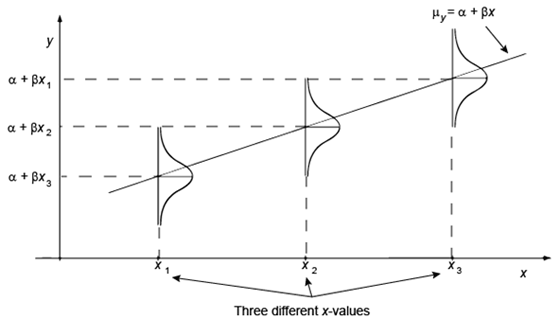
\includegraphics{images/conditionalmean.png}
http://www.learner.org/courses/againstallodds/about/glossary.html

\begin{itemize}
\tightlist
\item
  The goal is to estimate the coefficients (e.g. \(\beta_0\) and
  \(\beta_1\)). We represent the estimates of the coefficients with a
  "hat" on top of the letter.
\end{itemize}

\[ \hat{\beta}_0, \hat{\beta}_1 \]

\begin{itemize}
\tightlist
\item
  Once we estimate the coefficients \(\hat{\beta}_0\) and
  \(\hat{\beta}_1\), we can use these to predict new values of \(Y\)
  given new data \(X\).
\end{itemize}

\[\hat{y} = \hat{\beta}_0 + \hat{\beta}_1 x_1\]

\begin{itemize}
\tightlist
\item
  Multiple linear regression is when you have more than one independent
  variable and the estimation involves matrices

  \begin{itemize}
  \tightlist
  \item
    \(X_1\), \(X_2\), \(X_3\), \(\ldots\)
  \end{itemize}
\item
  How do you estimate the coefficients?

  \begin{itemize}
  \tightlist
  \item
    There are many ways to fit a linear regression model
  \item
    The method called \textbf{least squares} is the most common methods
  \item
    We will discuss least squares
  \end{itemize}
\end{itemize}

\[ Y = \beta_0 + \beta_1 X_1 + \ldots + \beta_p X_p + \epsilon\]

\subsubsection{\texorpdfstring{Estimating \(\hat\beta\): Least
squares}{Estimating \textbackslash{}hat\textbackslash{}beta: Least squares}}\label{estimating-hatbeta-least-squares}

\begin{center}\rule{0.5\linewidth}{\linethickness}\end{center}

\href{http://en.wikipedia.org/wiki/Least_squares}{Least squares} is a
method that can estimate the coefficients of a linear model by
minimizing the squared residuals:

\[ \mathscr{L} = \sum_{i=1}^N \epsilon_i = \sum_{i=1}^N \left( y_i - \hat{y}_i \right)^2  = \sum_{i=1}^N \left(y_i - \left(\beta_0 + \beta_1 x_i\right)\right)^2 \]

where \(N\) is the number of observations and \(\epsilon\) represents a
residual or error, ACTUAL - PREDICTED.

\paragraph{\texorpdfstring{Estimating the intercept \(\hat{\beta_0}\)
for the simple linear
model}{Estimating the intercept \textbackslash{}hat\{\textbackslash{}beta\_0\} for the simple linear model}}\label{estimating-the-intercept-hatbeta_0-for-the-simple-linear-model}

We want to minimize the squared residuals and solve for
\(\hat{\beta_0}\) so we take the partial derivative of \(\mathscr{L}\)
with respect to \(\hat{\beta_0}\)

    \$

\begin{align}
\frac{\partial \mathscr{L}}{\partial \hat{\beta_0}} &= \frac{\partial}{\partial \hat{\beta_0}} \sum_{i=1}^N \epsilon^2 \\
&= \frac{\partial}{\partial \hat{\beta_0}} \sum_{i=1}^N \left( y_i - \hat{y}_i \right)^2 \\
&= \frac{\partial}{\partial \hat{\beta_0}} \sum_{i=1}^N \left( y_i - \left( \hat{\beta}_0 + \hat{\beta}_1 x_i \right) \right)^2 \\
&= -2 \sum_{i=1}^N \left( y_i - \left( \hat{\beta}_0 + \hat{\beta}_1 x_i \right) \right) \hspace{25mm} \mbox{(by chain rule)} \\
&= -2 \sum_{i=1}^N y_i - \hat{\beta}_0 - \hat{\beta}_1 x_i \\
&= -2 \left[ \left( \sum_{i=1}^N y_i \right) - n \hat{\beta_0} - \hat{\beta}_1 \left( \sum_{i=1}^N x_i
\right) \right] \\
& 2 \left[ n \hat{\beta}_0 + \hat{\beta}_1 \sum_{i=1}^N x_i - \sum_{i=1}^N y_i \right] = 0 \hspace{20mm} \mbox{(Set equal to 0 and solve for $\hat{\beta}_0$)} \\
& n \hat{\beta}_0 + \hat{\beta}_1 \sum_{i=1}^N x_i - \sum{i=1}^N y_i = 0 \\
& n \hat{\beta}_0 = \sum_{i=1}^N y_i - \hat{\beta}_1 \sum_{i=1}^N x_i \\
& \hat{\beta}_0 = \frac{\sum_{i=1}^N y_i - \hat{\beta}_1 \sum_{i=1}^N x_i}{n} \\
& \hat{\beta}_0 = \frac{\sum_{i=1}^N y_i}{n} - \hat{\beta}_1 \frac{\sum_{i=1}^N x_i}{n} \\
& \boxed{\hat{\beta}_0 = \bar{y} - \hat{\beta}_1 \bar{x}}
\end{align}

\$

    Using this new information, we can compute the estimate for
\(\hat{\beta}_1\) by taking the partial derivative of \(\mathscr{L}\)
with respect to \(\hat{\beta}_1\).

    \$

\begin{align}
\frac{\partial \mathscr{L}}{\partial \hat{\beta_1}} &= \frac{\partial}{\partial \hat{\beta_1}} \sum_{i=1}^N \epsilon^2 \\
&= \frac{\partial}{\partial \hat{\beta_1}} \sum_{i=1}^N \left( y_i - \hat{y}_i \right)^2 \\
&= \frac{\partial}{\partial \hat{\beta_1}} \sum_{i=1}^N \left( y_i - \left( \hat{\beta}_0 + \hat{\beta}_1 x_i \right) \right)^2 \\
&= 2 \sum_{i=1}^N \left( y_i - \left( \hat{\beta}_0 + \hat{\beta}_1 x_i \right) \right) \left( -x_i \right) \hspace{25mm}\mbox{(by chain rule)} \\
&= -2 \sum_{i=1}^N x_i \left( y_i - \hat{\beta}_0 - \hat{\beta}_1 x_i \right) \\
&= -2 \sum_{i=1}^N x_i y_i - \hat{\beta}_0 x_i - \hat{\beta}_1 x_i^2 \\
&= -2 \sum_{i=1}^N x_i y_i - \left( \bar{y} - \hat{\beta}_1 \bar{x} \right) x_i - \hat{\beta}_1 x_i^2 \\
&= -2 \sum_{i=1}^N x_i y_i - \bar{y}x_i + \hat{\beta}_1\bar{x}x_i - \hat{\beta}_1 x_i^2 \\
&= -2 \left[ \sum_{i=1}^N x_i y_i - \bar{y} \sum_{i=1}^N x_i + \hat{\beta}_1\bar{x} - \hat{\beta}_1 x_i^2 \right] \\
&= -2 \left[ \hat{\beta}_1 \left\{ \bar{x} \sum_{i=1}^N x_i - \sum_{i=1}^N x_i^2 \right\} + \left\{ \sum_{i=1}^N x_i y_i - \bar{y} \sum_{i=1}^N x_i \right\}\right] \\
& 2 \left[ \hat{\beta}_1 \left\{ \sum_{i=1}^N x_i^2 - \bar{x} \sum_{i=1}^N x_i \right\} + \left\{ \bar{y} \sum_{i=1}^N x_i - \sum_{i=1}^N x_i y_i \right\} \right] = 0 \\
& \hat{\beta}_1 = \frac{-\left( \bar{y} \sum_{i=1}^N x_i - \sum_{i=1}^N x_i y_i \right)}{\sum_{i=1}^N x_i^2 - \bar{x}\sum_{i=1}^N x_i} \\
&= \frac{\sum_{i=1}^N x_i y_i - \bar{y} \sum_{i=1}^N x_i}{\sum_{i=1}^N x_i^2 - \bar{x} \sum_{i=1}^N x_i} \\
& \boxed{\hat{\beta}_1 = \frac{\sum_{i=1}^N x_i y_i - \bar{x}\bar{y}n}{\sum_{i=1}^N x_i^2 - n \bar{x}^2}}
\end{align}

\$

    The solution can be written in compact matrix notation as

\[\hat\beta =  (X^T X)^{-1}X^T Y\]

We wanted to show you this in case you remember linear algebra, in order
for this solution to exist we need \(X^T X\) to be invertible. Of course
this requires a few extra assumptions, \(X\) must be full rank so that
\(X^T X\) is invertible, etc. Basically, \(X^T X\) is full rank if all
rows and columns are linearly independent. This has a loose relationship
to variables and observations being independent respective. \textbf{This
is important for us because this means that having redundant features in
our regression models will lead to poorly fitting (and unstable)
models.} We'll see an implementation of this in the extra linear
regression example.

    \begin{center}\rule{0.5\linewidth}{\linethickness}\end{center}

\section{Part 2: Exploratory Data Analysis for Linear
Relationships}\label{part-2-exploratory-data-analysis-for-linear-relationships}

The \href{https://archive.ics.uci.edu/ml/datasets/Housing}{Boston
Housing data set} contains information about the housing values in
suburbs of Boston. This dataset was originally taken from the StatLib
library which is maintained at Carnegie Mellon University and is now
available on the UCI Machine Learning Repository.

\subsection{\texorpdfstring{Load the Boston Housing data set from
\texttt{sklearn}}{Load the Boston Housing data set from sklearn}}\label{load-the-boston-housing-data-set-from-sklearn}

\begin{center}\rule{0.5\linewidth}{\linethickness}\end{center}

This data set is available in the
\href{http://scikit-learn.org/stable/modules/generated/sklearn.datasets.load_boston.html\#sklearn.datasets.load_boston}{sklearn}
python module which is how we will access it today.

    \begin{Verbatim}[commandchars=\\\{\}]
{\color{incolor}In [{\color{incolor} }]:} \PY{k+kn}{from} \PY{n+nn}{sklearn}\PY{n+nn}{.}\PY{n+nn}{datasets} \PY{k}{import} \PY{n}{load\PYZus{}boston}
        \PY{k+kn}{import} \PY{n+nn}{pandas} \PY{k}{as} \PY{n+nn}{pd}
        
        \PY{n}{boston} \PY{o}{=} \PY{n}{load\PYZus{}boston}\PY{p}{(}\PY{p}{)}
\end{Verbatim}


    \begin{Verbatim}[commandchars=\\\{\}]
{\color{incolor}In [{\color{incolor} }]:} \PY{n}{boston}\PY{o}{.}\PY{n}{keys}\PY{p}{(}\PY{p}{)}
\end{Verbatim}


    \begin{Verbatim}[commandchars=\\\{\}]
{\color{incolor}In [{\color{incolor} }]:} \PY{n}{boston}\PY{o}{.}\PY{n}{data}\PY{o}{.}\PY{n}{shape}
\end{Verbatim}


    \begin{Verbatim}[commandchars=\\\{\}]
{\color{incolor}In [{\color{incolor} }]:} \PY{c+c1}{\PYZsh{} Print column names}
        \PY{n+nb}{print}\PY{p}{(}\PY{n}{boston}\PY{o}{.}\PY{n}{feature\PYZus{}names}\PY{p}{)}
\end{Verbatim}


    \begin{Verbatim}[commandchars=\\\{\}]
{\color{incolor}In [{\color{incolor} }]:} \PY{c+c1}{\PYZsh{} Print description of Boston housing data set}
        \PY{n+nb}{print}\PY{p}{(}\PY{n}{boston}\PY{o}{.}\PY{n}{DESCR}\PY{p}{)}
\end{Verbatim}


    Now let's explore the data set itself.

    \begin{Verbatim}[commandchars=\\\{\}]
{\color{incolor}In [{\color{incolor} }]:} \PY{n}{bos} \PY{o}{=} \PY{n}{pd}\PY{o}{.}\PY{n}{DataFrame}\PY{p}{(}\PY{n}{boston}\PY{o}{.}\PY{n}{data}\PY{p}{)}
        \PY{n}{bos}\PY{o}{.}\PY{n}{head}\PY{p}{(}\PY{p}{)}
\end{Verbatim}


    There are no column names in the DataFrame. Let's add those.

    \begin{Verbatim}[commandchars=\\\{\}]
{\color{incolor}In [{\color{incolor} }]:} \PY{n}{bos}\PY{o}{.}\PY{n}{columns} \PY{o}{=} \PY{n}{boston}\PY{o}{.}\PY{n}{feature\PYZus{}names}
        \PY{n}{bos}\PY{o}{.}\PY{n}{head}\PY{p}{(}\PY{p}{)}
\end{Verbatim}


    Now we have a pandas DataFrame called \texttt{bos} containing all the
data we want to use to predict Boston Housing prices. Let's create a
variable called \texttt{PRICE} which will contain the prices. This
information is contained in the \texttt{target} data.

    \begin{Verbatim}[commandchars=\\\{\}]
{\color{incolor}In [{\color{incolor} }]:} \PY{n+nb}{print}\PY{p}{(}\PY{n}{boston}\PY{o}{.}\PY{n}{target}\PY{o}{.}\PY{n}{shape}\PY{p}{)}
\end{Verbatim}


    \begin{Verbatim}[commandchars=\\\{\}]
{\color{incolor}In [{\color{incolor} }]:} \PY{n}{bos}\PY{p}{[}\PY{l+s+s1}{\PYZsq{}}\PY{l+s+s1}{PRICE}\PY{l+s+s1}{\PYZsq{}}\PY{p}{]} \PY{o}{=} \PY{n}{boston}\PY{o}{.}\PY{n}{target}
        \PY{n}{bos}\PY{o}{.}\PY{n}{head}\PY{p}{(}\PY{p}{)}
\end{Verbatim}


    \subsection{EDA and Summary
Statistics}\label{eda-and-summary-statistics}

\begin{center}\rule{0.5\linewidth}{\linethickness}\end{center}

Let's explore this data set. First we use \texttt{describe()} to get
basic summary statistics for each of the columns.

    \begin{Verbatim}[commandchars=\\\{\}]
{\color{incolor}In [{\color{incolor} }]:} \PY{n}{bos}\PY{o}{.}\PY{n}{describe}\PY{p}{(}\PY{p}{)}
\end{Verbatim}


    \subsubsection{Scatterplots}\label{scatterplots}

\begin{center}\rule{0.5\linewidth}{\linethickness}\end{center}

Let's look at some scatter plots for three variables: 'CRIM' (per capita
crime rate), 'RM' (number of rooms) and 'PTRATIO' (pupil-to-teacher
ratio in schools).

    \begin{Verbatim}[commandchars=\\\{\}]
{\color{incolor}In [{\color{incolor} }]:} \PY{n}{plt}\PY{o}{.}\PY{n}{scatter}\PY{p}{(}\PY{n}{bos}\PY{o}{.}\PY{n}{CRIM}\PY{p}{,} \PY{n}{bos}\PY{o}{.}\PY{n}{PRICE}\PY{p}{)}
        \PY{n}{plt}\PY{o}{.}\PY{n}{xlabel}\PY{p}{(}\PY{l+s+s2}{\PYZdq{}}\PY{l+s+s2}{Per capita crime rate by town (CRIM)}\PY{l+s+s2}{\PYZdq{}}\PY{p}{)}
        \PY{n}{plt}\PY{o}{.}\PY{n}{ylabel}\PY{p}{(}\PY{l+s+s2}{\PYZdq{}}\PY{l+s+s2}{Housing Price}\PY{l+s+s2}{\PYZdq{}}\PY{p}{)}
        \PY{n}{plt}\PY{o}{.}\PY{n}{title}\PY{p}{(}\PY{l+s+s2}{\PYZdq{}}\PY{l+s+s2}{Relationship between CRIM and Price}\PY{l+s+s2}{\PYZdq{}}\PY{p}{)}
\end{Verbatim}


    Part 2 Checkup Exercise Set I

Exercise: What kind of relationship do you see? e.g. positive, negative?
linear? non-linear? Is there anything else strange or interesting about
the data? What about outliers?

Exercise: Create scatter plots between \emph{RM} and \emph{PRICE}, and
\emph{PTRATIO} and \emph{PRICE}. Label your axes appropriately using
human readable labels. Tell a story about what you see.

Exercise: What are some other numeric variables of interest? Why do you
think they are interesting? Plot scatterplots with these variables and
\emph{PRICE} (house price) and tell a story about what you see.

    \begin{Verbatim}[commandchars=\\\{\}]
{\color{incolor}In [{\color{incolor} }]:} \PY{c+c1}{\PYZsh{} your turn: describe relationship}
\end{Verbatim}


    \begin{Verbatim}[commandchars=\\\{\}]
{\color{incolor}In [{\color{incolor} }]:} \PY{c+c1}{\PYZsh{} your turn: scatter plot between *RM* and *PRICE*}
\end{Verbatim}


    \begin{Verbatim}[commandchars=\\\{\}]
{\color{incolor}In [{\color{incolor} }]:} \PY{c+c1}{\PYZsh{} your turn: scatter plot between *PTRATIO* and *PRICE*}
\end{Verbatim}


    \begin{Verbatim}[commandchars=\\\{\}]
{\color{incolor}In [{\color{incolor} }]:} \PY{c+c1}{\PYZsh{} your turn: create some other scatter plots}
\end{Verbatim}


    \subsubsection{Scatterplots using
Seaborn}\label{scatterplots-using-seaborn}

\begin{center}\rule{0.5\linewidth}{\linethickness}\end{center}

\href{https://stanford.edu/~mwaskom/software/seaborn/}{Seaborn} is a
cool Python plotting library built on top of matplotlib. It provides
convenient syntax and shortcuts for many common types of plots, along
with better-looking defaults.

We can also use
\href{https://stanford.edu/~mwaskom/software/seaborn/tutorial/regression.html\#functions-to-draw-linear-regression-models}{seaborn
regplot} for the scatterplot above. This provides automatic linear
regression fits (useful for data exploration later on). Here's one
example below.

    \begin{Verbatim}[commandchars=\\\{\}]
{\color{incolor}In [{\color{incolor} }]:} \PY{n}{sns}\PY{o}{.}\PY{n}{regplot}\PY{p}{(}\PY{n}{y}\PY{o}{=}\PY{l+s+s2}{\PYZdq{}}\PY{l+s+s2}{PRICE}\PY{l+s+s2}{\PYZdq{}}\PY{p}{,} \PY{n}{x}\PY{o}{=}\PY{l+s+s2}{\PYZdq{}}\PY{l+s+s2}{RM}\PY{l+s+s2}{\PYZdq{}}\PY{p}{,} \PY{n}{data}\PY{o}{=}\PY{n}{bos}\PY{p}{,} \PY{n}{fit\PYZus{}reg} \PY{o}{=} \PY{k+kc}{True}\PY{p}{)}
\end{Verbatim}


    \subsubsection{Histograms}\label{histograms}

\begin{center}\rule{0.5\linewidth}{\linethickness}\end{center}

    \begin{Verbatim}[commandchars=\\\{\}]
{\color{incolor}In [{\color{incolor} }]:} \PY{n}{plt}\PY{o}{.}\PY{n}{hist}\PY{p}{(}\PY{n}{np}\PY{o}{.}\PY{n}{log}\PY{p}{(}\PY{n}{bos}\PY{o}{.}\PY{n}{CRIM}\PY{p}{)}\PY{p}{)}
        \PY{n}{plt}\PY{o}{.}\PY{n}{title}\PY{p}{(}\PY{l+s+s2}{\PYZdq{}}\PY{l+s+s2}{CRIM}\PY{l+s+s2}{\PYZdq{}}\PY{p}{)}
        \PY{n}{plt}\PY{o}{.}\PY{n}{xlabel}\PY{p}{(}\PY{l+s+s2}{\PYZdq{}}\PY{l+s+s2}{Crime rate per capita}\PY{l+s+s2}{\PYZdq{}}\PY{p}{)}
        \PY{n}{plt}\PY{o}{.}\PY{n}{ylabel}\PY{p}{(}\PY{l+s+s2}{\PYZdq{}}\PY{l+s+s2}{Frequencey}\PY{l+s+s2}{\PYZdq{}}\PY{p}{)}
        \PY{n}{plt}\PY{o}{.}\PY{n}{show}\PY{p}{(}\PY{p}{)}
\end{Verbatim}


    Part 2 Checkup Exercise Set II

Exercise: In the above histogram, we took the logarithm of the crime
rate per capita. Repeat this histogram without taking the log. What was
the purpose of taking the log? What do we gain by making this
transformation? What do you now notice about this variable that is not
obvious without making the transformation?

Exercise: Plot histograms for \emph{RM} and \emph{PTRATIO}, along with
the two variables you picked in the previous section.

    \begin{Verbatim}[commandchars=\\\{\}]
{\color{incolor}In [{\color{incolor} }]:} \PY{c+c1}{\PYZsh{}your turn}
\end{Verbatim}


    \subsection{Part 3: Linear Regression with Boston Housing Data
Example}\label{part-3-linear-regression-with-boston-housing-data-example}

\begin{center}\rule{0.5\linewidth}{\linethickness}\end{center}

Here,

\(Y\) = boston housing prices (called "target" data in python, and
referred to as the dependent variable or response variable)

and

\(X\) = all the other features (or independent variables, predictors or
explanatory variables)

which we will use to fit a linear regression model and predict Boston
housing prices. We will use the least-squares method to estimate the
coefficients.

    We'll use two ways of fitting a linear regression. We recommend the
first but the second is also powerful in its features.

    \subsubsection{\texorpdfstring{Fitting Linear Regression using
\texttt{statsmodels}}{Fitting Linear Regression using statsmodels}}\label{fitting-linear-regression-using-statsmodels}

\begin{center}\rule{0.5\linewidth}{\linethickness}\end{center}

\href{http://statsmodels.sourceforge.net/}{Statsmodels} is a great
Python library for a lot of basic and inferential statistics. It also
provides basic regression functions using an R-like syntax, so it's
commonly used by statisticians. While we don't cover statsmodels
officially in the Data Science Intensive workshop, it's a good library
to have in your toolbox. Here's a quick example of what you could do
with it. The version of least-squares we will use in statsmodels is
called \emph{ordinary least-squares (OLS)}. There are many other
versions of least-squares such as
\href{https://en.wikipedia.org/wiki/Partial_least_squares_regression}{partial
least squares (PLS)} and
\href{https://en.wikipedia.org/wiki/Iteratively_reweighted_least_squares}{weighted
least squares (WLS)}.

    \begin{Verbatim}[commandchars=\\\{\}]
{\color{incolor}In [{\color{incolor} }]:} \PY{c+c1}{\PYZsh{} Import regression modules}
        \PY{k+kn}{import} \PY{n+nn}{statsmodels}\PY{n+nn}{.}\PY{n+nn}{api} \PY{k}{as} \PY{n+nn}{sm}
        \PY{k+kn}{from} \PY{n+nn}{statsmodels}\PY{n+nn}{.}\PY{n+nn}{formula}\PY{n+nn}{.}\PY{n+nn}{api} \PY{k}{import} \PY{n}{ols}
\end{Verbatim}


    \begin{Verbatim}[commandchars=\\\{\}]
{\color{incolor}In [{\color{incolor} }]:} \PY{c+c1}{\PYZsh{} statsmodels works nicely with pandas dataframes}
        \PY{c+c1}{\PYZsh{} The thing inside the \PYZdq{}quotes\PYZdq{} is called a formula, a bit on that below}
        \PY{n}{m} \PY{o}{=} \PY{n}{ols}\PY{p}{(}\PY{l+s+s1}{\PYZsq{}}\PY{l+s+s1}{PRICE \PYZti{} RM}\PY{l+s+s1}{\PYZsq{}}\PY{p}{,}\PY{n}{bos}\PY{p}{)}\PY{o}{.}\PY{n}{fit}\PY{p}{(}\PY{p}{)}
        \PY{n+nb}{print}\PY{p}{(}\PY{n}{m}\PY{o}{.}\PY{n}{summary}\PY{p}{(}\PY{p}{)}\PY{p}{)}
\end{Verbatim}


    \paragraph{Interpreting coefficients}\label{interpreting-coefficients}

There is a ton of information in this output. But we'll concentrate on
the coefficient table (middle table). We can interpret the \texttt{RM}
coefficient (9.1021) by first noticing that the p-value (under
\texttt{P\textgreater{}\textbar{}t\textbar{}}) is so small, basically
zero. This means that the number of rooms, \texttt{RM}, is a
statisticall significant predictor of \texttt{PRICE}. The regression
coefficient for \texttt{RM} of 9.1021 means that \emph{on average, each
additional room is associated with an increase of \(\$9,100\) in house
price net of the other variables}. The confidence interval gives us a
range of plausible values for this average change, about
(\(\$8,279, \$9,925\)), definitely not chump change.

In general, the \(\hat{\beta_i}, i > 0\) can be interpreted as the
following: "A one unit increase in \(x_i\) is associated with, on
average, a \(\hat{\beta_i}\) increase/decrease in \(y\) net of all other
variables."

On the other hand, the interpretation for the intercept,
\(\hat{\beta}_0\) is the average of \(y\) given that all of the
independent variables \(x_i\) are 0.

    \paragraph{\texorpdfstring{\texttt{statsmodels}
formulas}{statsmodels formulas}}\label{statsmodels-formulas}

\begin{center}\rule{0.5\linewidth}{\linethickness}\end{center}

This formula notation will seem familiar to \texttt{R} users, but will
take some getting used to for people coming from other languages or are
new to statistics.

The formula gives instruction for a general structure for a regression
call. For \texttt{statsmodels} (\texttt{ols} or \texttt{logit}) calls
you need to have a Pandas dataframe with column names that you will add
to your formula. In the below example you need a pandas data frame that
includes the columns named (\texttt{Outcome}, \texttt{X1},\texttt{X2},
...), but you don't need to build a new dataframe for every regression.
Use the same dataframe with all these things in it. The structure is
very simple:

\texttt{Outcome\ \textasciitilde{}\ X1}

But of course we want to to be able to handle more complex models, for
example multiple regression is doone like this:

\texttt{Outcome\ \textasciitilde{}\ X1\ +\ X2\ +\ X3}

In general, a formula for an OLS multiple linear regression is

\texttt{Y\ \textasciitilde{}\ X1\ +\ X2\ +\ ...\ +\ Xp}

This is the very basic structure but it should be enough to get you
through the homework. Things can get much more complex. You can force
statsmodels to treat variables as categorical with the \texttt{C()}
function, call numpy functions to transform data such as \texttt{np.log}
for extremely-skewed data, or fit a model without an intercept by
including \texttt{-\ 1} in the formula. For a quick run-down of further
uses see the \texttt{statsmodels}
\href{http://statsmodels.sourceforge.net/devel/example_formulas.html}{help
page}.

    Let's see how our model actually fit our data. We can see below that
there is a ceiling effect, we should probably look into that. Also, for
large values of \(Y\) we get underpredictions, most predictions are
below the 45-degree gridlines.

    Part 3 Checkup Exercise Set I

Exercise: Create a scatterplot between the predicted prices, available
in \texttt{m.fittedvalues} (where \texttt{m} is the fitted model) and
the original prices. How does the plot look? Do you notice anything
interesting or weird in the plot? Comment on what you see.

    \begin{Verbatim}[commandchars=\\\{\}]
{\color{incolor}In [{\color{incolor} }]:} \PY{c+c1}{\PYZsh{} your turn}
\end{Verbatim}


    \subsubsection{\texorpdfstring{Fitting Linear Regression using
\texttt{sklearn}}{Fitting Linear Regression using sklearn}}\label{fitting-linear-regression-using-sklearn}

    \begin{Verbatim}[commandchars=\\\{\}]
{\color{incolor}In [{\color{incolor} }]:} \PY{k+kn}{from} \PY{n+nn}{sklearn}\PY{n+nn}{.}\PY{n+nn}{linear\PYZus{}model} \PY{k}{import} \PY{n}{LinearRegression}
        \PY{n}{X} \PY{o}{=} \PY{n}{bos}\PY{o}{.}\PY{n}{drop}\PY{p}{(}\PY{l+s+s1}{\PYZsq{}}\PY{l+s+s1}{PRICE}\PY{l+s+s1}{\PYZsq{}}\PY{p}{,} \PY{n}{axis} \PY{o}{=} \PY{l+m+mi}{1}\PY{p}{)}
        
        \PY{c+c1}{\PYZsh{} This creates a LinearRegression object}
        \PY{n}{lm} \PY{o}{=} \PY{n}{LinearRegression}\PY{p}{(}\PY{p}{)}
        \PY{n}{lm}
\end{Verbatim}


    \paragraph{What can you do with a LinearRegression
object?}\label{what-can-you-do-with-a-linearregression-object}

\begin{center}\rule{0.5\linewidth}{\linethickness}\end{center}

Check out the scikit-learn
\href{http://scikit-learn.org/stable/modules/generated/sklearn.linear_model.LinearRegression.html}{docs
here}. We have listed the main functions here. Most machine learning
models in scikit-learn follow this same API of fitting a model with
\texttt{fit}, making predictions with \texttt{predict} and the
appropriate scoring function \texttt{score} for each model.

    \begin{longtable}[]{@{}ll@{}}
\toprule
\begin{minipage}[b]{0.05\columnwidth}\raggedright\strut
Main functions\strut
\end{minipage} & \begin{minipage}[b]{0.05\columnwidth}\raggedright\strut
Description\strut
\end{minipage}\tabularnewline
\midrule
\endhead
\begin{minipage}[t]{0.05\columnwidth}\raggedright\strut
\texttt{lm.fit()}\strut
\end{minipage} & \begin{minipage}[t]{0.05\columnwidth}\raggedright\strut
Fit a linear model\strut
\end{minipage}\tabularnewline
\begin{minipage}[t]{0.05\columnwidth}\raggedright\strut
\texttt{lm.predit()}\strut
\end{minipage} & \begin{minipage}[t]{0.05\columnwidth}\raggedright\strut
Predict Y using the linear model with estimated coefficients\strut
\end{minipage}\tabularnewline
\begin{minipage}[t]{0.05\columnwidth}\raggedright\strut
\texttt{lm.score()}\strut
\end{minipage} & \begin{minipage}[t]{0.05\columnwidth}\raggedright\strut
Returns the coefficient of determination (R\^{}2). \emph{A measure of
how well observed outcomes are replicated by the model, as the
proportion of total variation of outcomes explained by the model}\strut
\end{minipage}\tabularnewline
\bottomrule
\end{longtable}

    \paragraph{What output can you get?}\label{what-output-can-you-get}

    \begin{Verbatim}[commandchars=\\\{\}]
{\color{incolor}In [{\color{incolor} }]:} \PY{c+c1}{\PYZsh{} Look inside lm object}
        \PY{c+c1}{\PYZsh{} lm.\PYZlt{}tab\PYZgt{}}
\end{Verbatim}


    \begin{longtable}[]{@{}ll@{}}
\toprule
Output & Description\tabularnewline
\midrule
\endhead
\texttt{lm.coef\_} & Estimated coefficients\tabularnewline
\texttt{lm.intercept\_} & Estimated intercept\tabularnewline
\bottomrule
\end{longtable}

    \subsubsection{Fit a linear model}\label{fit-a-linear-model}

\begin{center}\rule{0.5\linewidth}{\linethickness}\end{center}

The \texttt{lm.fit()} function estimates the coefficients the linear
regression using least squares.

    \begin{Verbatim}[commandchars=\\\{\}]
{\color{incolor}In [{\color{incolor} }]:} \PY{c+c1}{\PYZsh{} Use all 13 predictors to fit linear regression model}
        \PY{n}{lm}\PY{o}{.}\PY{n}{fit}\PY{p}{(}\PY{n}{X}\PY{p}{,} \PY{n}{bos}\PY{o}{.}\PY{n}{PRICE}\PY{p}{)}
\end{Verbatim}


    Part 3 Checkup Exercise Set II

Exercise: How would you change the model to not fit an intercept term?
Would you recommend not having an intercept? Why or why not? For more
information on why to include or exclude an intercept, look
\href{https://online.stat.psu.edu/~ajw13/stat501/SpecialTopics/Reg_thru_origin.pdf}{here}.

Exercise: One of the assumptions of the linear model is that the
residuals must be i.i.d. (independently and identically distributed). To
satisfy this, is it enough that the residuals are normally distributed?
Explain your answer.

Exercise: True or false. To use linear regression, \(Y\) must be
normally distributed. Explain your answer.

    \begin{Verbatim}[commandchars=\\\{\}]
{\color{incolor}In [{\color{incolor} }]:} \PY{c+c1}{\PYZsh{} your turn}
\end{Verbatim}


    \subsubsection{Estimated intercept and
coefficients}\label{estimated-intercept-and-coefficients}

Let's look at the estimated coefficients from the linear model using
\texttt{1m.intercept\_} and \texttt{lm.coef\_}.

After we have fit our linear regression model using the least squares
method, we want to see what are the estimates of our coefficients
\(\beta_0\), \(\beta_1\), ..., \(\beta_{13}\):

\[ \hat{\beta}_0, \hat{\beta}_1, \ldots, \hat{\beta}_{13} \]

    \begin{Verbatim}[commandchars=\\\{\}]
{\color{incolor}In [{\color{incolor} }]:} \PY{n+nb}{print}\PY{p}{(}\PY{l+s+s1}{\PYZsq{}}\PY{l+s+s1}{Estimated intercept coefficient: }\PY{l+s+si}{\PYZob{}\PYZcb{}}\PY{l+s+s1}{\PYZsq{}}\PY{o}{.}\PY{n}{format}\PY{p}{(}\PY{n}{lm}\PY{o}{.}\PY{n}{intercept\PYZus{}}\PY{p}{)}\PY{p}{)}
\end{Verbatim}


    \begin{Verbatim}[commandchars=\\\{\}]
{\color{incolor}In [{\color{incolor} }]:} \PY{n+nb}{print}\PY{p}{(}\PY{l+s+s1}{\PYZsq{}}\PY{l+s+s1}{Number of coefficients: }\PY{l+s+si}{\PYZob{}\PYZcb{}}\PY{l+s+s1}{\PYZsq{}}\PY{o}{.}\PY{n}{format}\PY{p}{(}\PY{n+nb}{len}\PY{p}{(}\PY{n}{lm}\PY{o}{.}\PY{n}{coef\PYZus{}}\PY{p}{)}\PY{p}{)}\PY{p}{)}
\end{Verbatim}


    \begin{Verbatim}[commandchars=\\\{\}]
{\color{incolor}In [{\color{incolor} }]:} \PY{c+c1}{\PYZsh{} The coefficients}
        \PY{n}{pd}\PY{o}{.}\PY{n}{DataFrame}\PY{p}{(}\PY{p}{\PYZob{}}\PY{l+s+s1}{\PYZsq{}}\PY{l+s+s1}{features}\PY{l+s+s1}{\PYZsq{}}\PY{p}{:} \PY{n}{X}\PY{o}{.}\PY{n}{columns}\PY{p}{,} \PY{l+s+s1}{\PYZsq{}}\PY{l+s+s1}{estimatedCoefficients}\PY{l+s+s1}{\PYZsq{}}\PY{p}{:} \PY{n}{lm}\PY{o}{.}\PY{n}{coef\PYZus{}}\PY{p}{\PYZcb{}}\PY{p}{)}\PY{p}{[}\PY{p}{[}\PY{l+s+s1}{\PYZsq{}}\PY{l+s+s1}{features}\PY{l+s+s1}{\PYZsq{}}\PY{p}{,} \PY{l+s+s1}{\PYZsq{}}\PY{l+s+s1}{estimatedCoefficients}\PY{l+s+s1}{\PYZsq{}}\PY{p}{]}\PY{p}{]}
\end{Verbatim}


    \subsubsection{Predict Prices}\label{predict-prices}

We can calculate the predicted prices (\(\hat{Y}_i\)) using
\texttt{lm.predict}.

\[ \hat{Y}_i = \hat{\beta}_0 + \hat{\beta}_1 X_1 + \ldots \hat{\beta}_{13} X_{13} \]

    \begin{Verbatim}[commandchars=\\\{\}]
{\color{incolor}In [{\color{incolor} }]:} \PY{c+c1}{\PYZsh{} first five predicted prices}
        \PY{n}{lm}\PY{o}{.}\PY{n}{predict}\PY{p}{(}\PY{n}{X}\PY{p}{)}\PY{p}{[}\PY{l+m+mi}{0}\PY{p}{:}\PY{l+m+mi}{5}\PY{p}{]}
\end{Verbatim}


    Part 3 Checkup Exercise Set III

Exercise: Histogram: Plot a histogram of all the predicted prices. Write
a story about what you see. Describe the shape, center and spread of the
distribution. Are there any outliers? What might be the reason for them?
Should we do anything special with them?

Exercise: Scatterplot: Let's plot the true prices compared to the
predicted prices to see they disagree (we did this with
\texttt{statsmodels} before).

Exercise: We have looked at fitting a linear model in both
\texttt{statsmodels} and \texttt{scikit-learn}. What are the advantages
and disadvantages of each based on your exploration? Based on the
information provided by both packages, what advantage does
\texttt{statsmodels} provide?

    \begin{Verbatim}[commandchars=\\\{\}]
{\color{incolor}In [{\color{incolor} }]:} \PY{c+c1}{\PYZsh{} your turn}
\end{Verbatim}


    \subsubsection{Evaluating the Model:
Sum-of-Squares}\label{evaluating-the-model-sum-of-squares}

The partitioning of the sum-of-squares shows the variance in the
predictions explained by the model and the variance that is attributed
to error.

\[TSS = ESS + RSS\]

\paragraph{\texorpdfstring{Residual Sum-of-Squares (aka
\(RSS\))}{Residual Sum-of-Squares (aka RSS)}}\label{residual-sum-of-squares-aka-rss}

The residual sum-of-squares is one of the basic ways of quantifying how
much error exists in the fitted model. We will revisit this in a bit.

\[ RSS = \sum_{i=1}^N r_i^2 = \sum_{i=1}^N \left(y_i - \left(\beta_0 + \beta_1 x_i\right)\right)^2 \]

    \begin{Verbatim}[commandchars=\\\{\}]
{\color{incolor}In [{\color{incolor} }]:} \PY{n+nb}{print}\PY{p}{(}\PY{n}{np}\PY{o}{.}\PY{n}{sum}\PY{p}{(}\PY{p}{(}\PY{n}{bos}\PY{o}{.}\PY{n}{PRICE} \PY{o}{\PYZhy{}} \PY{n}{lm}\PY{o}{.}\PY{n}{predict}\PY{p}{(}\PY{n}{X}\PY{p}{)}\PY{p}{)} \PY{o}{*}\PY{o}{*} \PY{l+m+mi}{2}\PY{p}{)}\PY{p}{)}
\end{Verbatim}


    \paragraph{\texorpdfstring{Explained Sum-of-Squares (aka
\(ESS\))}{Explained Sum-of-Squares (aka ESS)}}\label{explained-sum-of-squares-aka-ess}

The explained sum-of-squares measures the variance explained by the
regression model.

\[ESS = \sum_{i=1}^N \left( \hat{y}_i - \bar{y} \right)^2 = \sum_{i=1}^N \left( \left( \hat{\beta}_0 + \hat{\beta}_1 x_i \right) - \bar{y} \right)^2\]

    \begin{Verbatim}[commandchars=\\\{\}]
{\color{incolor}In [{\color{incolor} }]:} \PY{n+nb}{print}\PY{p}{(}\PY{n}{np}\PY{o}{.}\PY{n}{sum}\PY{p}{(}\PY{n}{lm}\PY{o}{.}\PY{n}{predict}\PY{p}{(}\PY{n}{X}\PY{p}{)} \PY{o}{\PYZhy{}} \PY{n}{np}\PY{o}{.}\PY{n}{mean}\PY{p}{(}\PY{n}{bos}\PY{o}{.}\PY{n}{PRICE}\PY{p}{)}\PY{p}{)} \PY{o}{*}\PY{o}{*} \PY{l+m+mi}{2}\PY{p}{)}
\end{Verbatim}


    \subsubsection{\texorpdfstring{Evaluating the Model: The Coefficient of
Determination
(\(R^2\))}{Evaluating the Model: The Coefficient of Determination (R\^{}2)}}\label{evaluating-the-model-the-coefficient-of-determination-r2}

The coefficient of determination, \(R^2\), tells us the percentage of
the variance in the response variable \(Y\) that can be explained by the
linear regression model.

\[ R^2 = \frac{ESS}{TSS} \]

The \(R^2\) value is one of the most common metrics that people use in
describing the quality of a model, but it is important to note that
\emph{\(R^2\) increases artificially as a side-effect of increasing the
number of independent variables.} While \(R^2\) is reported in almost
all statistical packages, another metric called the \emph{adjusted
\(R^2\)} is also provided as it takes into account the number of
variables in the model, and can sometimes even be used for non-linear
regression models!

\[R_{adj}^2 = 1 - \left( 1 - R^2 \right) \frac{N - 1}{N - K - 1} = R^2 - \left( 1 - R^2 \right) \frac{K}{N - K - 1} = 1 - \frac{\frac{RSS}{DF_R}}{\frac{TSS}{DF_T}}\]

where \(N\) is the number of observations, \(K\) is the number of
variables, \(DF_R = N - K - 1\) is the degrees of freedom associated
with the residual error and \(DF_T = N - 1\) is the degrees of the
freedom of the total error.

    \subsubsection{\texorpdfstring{Evaluating the Model: Mean Squared Error
and the
\(F\)-Statistic}{Evaluating the Model: Mean Squared Error and the F-Statistic}}\label{evaluating-the-model-mean-squared-error-and-the-f-statistic}

\begin{center}\rule{0.5\linewidth}{\linethickness}\end{center}

The mean squared errors are just the \emph{averages} of the
sum-of-squares errors over their respective degrees of freedom.

\[MSE = \frac{ESS}{K}\] \[MSR = \frac{RSS}{N-K-1}\]

\textbf{Remember: } Notation may vary across resources particularly the
use of \emph{R} and \emph{E} in \emph{RSS/ESS} and \emph{MSR/MSE}. In
some resources, E = explained and R = residual. In other resources, E =
error and R = regression (explained). \textbf{This is a very important
distinction that requires looking at the formula to determine which
naming scheme is being used.}

Given the MSR and MSE, we can now determine whether or not the entire
model we just fit is even statistically significant. We use an
\(F\)-test for this. The null hypothesis is that all of the \(\beta\)
coefficients are zero, that is, none of them have any effect on \(Y\).
The alternative is that \emph{at least one} \(\beta\) coefficient is
nonzero, but it doesn't tell us which one in a multiple regression:

\[H_0: \beta_i = 0, \mbox{for all $i$} \\
H_A: \beta_i > 0, \mbox{for some $i$}\]

\[F = \frac{MSR}{MSE} = \left( \frac{R^2}{1 - R^2} \right) \left( \frac{N - K - 1}{K} \right)\]

Once we compute the \(F\)-statistic, we can use the \(F\)-distribution
with \(N-K\) and \(K-1\) degrees of degrees of freedom to get a p-value.

\textbf{Warning!} The \(F\)-statistic mentioned in this section is NOT
the same as the F1-measure or F1-value discused in Unit 7.

    Part 3 Checkup Exercise Set IV

Let's look at the relationship between \texttt{PTRATIO} and housing
price.

Exercise: Make a scatterplot of \texttt{PTRATIO} and housing price. Tell
a story about the relationship between the variables.

Exercise: Try fitting a linear regression model using only the 'PTRATIO'
(pupil-teacher ratio by town) and interpret the intercept and the
coefficients.

Exercise: Calculate (or extract) the \(R^2\) value. What does it tell
you?

Exercise: Compute the \(F\)-statistic. What does it tell you?

Exercise: Take a close look at the \(F\)-statistic and the
\(t\)-statistic for the regression coefficient. What relationship do you
notice? Note that this relationship only applies in \emph{simple} linear
regression models.

    \begin{Verbatim}[commandchars=\\\{\}]
{\color{incolor}In [{\color{incolor} }]:} \PY{c+c1}{\PYZsh{} your turn}
\end{Verbatim}


    Part 3 Checkup Exercise Set V

Fit a linear regression model using three independent variables

'CRIM' (per capita crime rate by town)

'RM' (average number of rooms per dwelling)

'PTRATIO' (pupil-teacher ratio by town)

Exercise: Compute or extract the \(F\)-statistic. What does it tell you
about the model?

Exercise: Compute or extract the \(R^2\) statistic. What does it tell
you about the model?

Exercise: Which variables in the model are significant in predicting
house price? Write a story that interprets the coefficients.

    \begin{Verbatim}[commandchars=\\\{\}]
{\color{incolor}In [{\color{incolor} }]:} \PY{c+c1}{\PYZsh{} your turn}
\end{Verbatim}


    \subsection{Part 4: Comparing Models}\label{part-4-comparing-models}

    During modeling, there will be times when we want to compare models to
see which one is more predictive or fits the data better. There are many
ways to compare models, but we will focus on two.

    \subsubsection{\texorpdfstring{The \(F\)-Statistic
Revisited}{The F-Statistic Revisited}}\label{the-f-statistic-revisited}

The \(F\)-statistic can also be used to compare two \emph{nested}
models, that is, two models trained on the same dataset where one of the
models contains a \emph{subset} of the variables of the other model. The
\emph{full} model contains \(K\) variables and the \emph{reduced} model
contains a subset of these \(K\) variables. This allows us to add
additional variables to a base model and then test if adding the
variables helped the model fit.

\[F = \frac{\left( \frac{RSS_{full} - RSS_{reduced}}{K_{full} - K_{reduced}} \right)}{\left( \frac{RSS_{reduced}}{N - K_{reduced}} \right)}\]

    \subsubsection{Akaike Information Criterion
(AIC)}\label{akaike-information-criterion-aic}

Another statistic for comparing two models is AIC, which is based on the
likelihood function and takes into account the number of variables in
the model.

\[AIC = 2 K - 2 \log_e{L}\]

where \(L\) is the likelihood of the model. AIC is meaningless in the
absolute sense, and is only meaningful when compared to AIC values from
other models. Lower values of AIC indicate better fitting models.

\texttt{statsmodels} provides the AIC in its output.

    Part 4 Checkup Exercises

Exercise: Find another variable (or two) to add to the model we built in
Part 3. Compute the \(F\)-test comparing the two models as well as the
AIC. Which model is better?

    \subsection{Part 5: Evaluating the Model via Model Assumptions and Other
Issues}\label{part-5-evaluating-the-model-via-model-assumptions-and-other-issues}

\begin{center}\rule{0.5\linewidth}{\linethickness}\end{center}

Linear regression makes several assumptions. It is always best to check
that these assumptions are valid after fitting a linear regression
model.

\textbf{Linearity}. The dependent variable \(Y\) is a linear combination
of the regression coefficients and the independent variables \(X\). This
can be verified with a scatterplot of each \(X\) vs. \(Y\) and plotting
correlations among \(X\). Nonlinearity can sometimes be resolved by
\href{https://onlinecourses.science.psu.edu/stat501/node/318}{transforming}
one or more independent variables, the dependent variable, or both. In
other cases, a
\href{https://en.wikipedia.org/wiki/Generalized_linear_model}{generalized
linear model} or a
\href{https://en.wikipedia.org/wiki/Nonlinear_regression}{nonlinear
model} may be warranted.

\textbf{Constant standard deviation}. The SD of the dependent variable
\(Y\) should be constant for different values of X. We can check this by
plotting each \(X\) against \(Y\) and verifying that there is no
"funnel" shape showing data points fanning out as \(X\) increases or
decreases. Some techniques for dealing with non-constant variance
include weighted least squares (WLS),
\href{https://en.wikipedia.org/wiki/Heteroscedasticity-consistent_standard_errors}{robust
standard errors}, or variance stabilizing transformations.

\textbf{Normal distribution for errors}. The \(\epsilon\) term we
discussed at the beginning are assumed to be normally distributed. This
can be verified with a fitted values vs. residuals plot and verifying
that there is no pattern, and with a quantile plot.
\[ \epsilon_i \sim N(0, \sigma^2)\] Sometimes the distributions of
responses \(Y\) may not be normally distributed at any given value of
\(X\). e.g. skewed positively or negatively.

\textbf{Independent errors}. The observations are assumed to be obtained
independently.

\begin{verbatim}
    <li>e.g. Observations across time may be correlated
</ul>
\end{verbatim}

There are some other issues that are important investigate with linear
regression models.

\textbf{Correlated Predictors:} Care should be taken to make sure that
the independent variables in a regression model are not too highly
correlated. Correlated predictors typically do not majorly affect
prediction, but do inflate standard errors of coefficients making
interpretation unreliable. Common solutions are dropping the least
important variables involved in the correlations, using regularlization,
or, when many predictors are highly correlated, considering a dimension
reduction technique such as principal component analysis (PCA).

\textbf{Influential Points:} Data points that have undue influence on
the regression model. These points can be high leverage points or
outliers. Such points are typically removed and the regression model
rerun.

    Part 5 Checkup Exercises

Take the reduced model from Part 3 to answer the following exercises.
Take a look at
\href{http://mpastell.com/2013/04/19/python_regression/}{this blog post}
for more information on using statsmodels to construct these plots.

Exercise: Construct a fitted values versus residuals plot. What does the
plot tell you? Are there any violations of the model assumptions?

Exercise: Construct a quantile plot of the residuals. What does the plot
tell you?

Exercise: What are some advantages and disadvantages of the fitted vs.
residual and quantile plot compared to each other?

Exercise: Identify any outliers (if any) in your model and write a story
describing what these outliers might represent.

Exercise: Construct a leverage plot and identify high leverage points in
the model. Write a story explaining possible reasons for the high
leverage points.

Exercise: Remove the outliers and high leverage points from your model
and run the regression again. How do the results change?

    \begin{Verbatim}[commandchars=\\\{\}]
{\color{incolor}In [{\color{incolor} }]:} \PY{c+c1}{\PYZsh{} Your turn.}
\end{Verbatim}



    % Add a bibliography block to the postdoc
    
    
    
    \end{document}
